\documentclass[../main.tex]{subfiles}

\begin{document}

    \section{}
Old vs new
----------

Dans les "anciennes" théories du bien être, l'utilité est comprise comme un
concept cardinal et comparable entre les individus. La théorie cardinale suppose
qu'il y a une échelle absolue de l'utilité et que l'on peut interpréter la
différence d'utilité entre deux situations quantitativement. Autrement,
si dans une situation X l'utilité d'un agent est U(X) = 20, et dans une situation
Y, son utilité est U(Y) = 40, cela a un sens d'affirmer que l'individu est plus
heureux de 20 unités d'utilité dans la seconde situation, ou qu'il est deux fois
plus heureux dans la seconde situation. Une étape supplémentaire est de considérer
que l'on peut comparer les utilités de deux agents, i.e. si un agent A a une
utilité U_A = 50 et un agent B a une utilité U_B = 100, on peut dire que l'agent
B est deux fois plus heureux. C'est ce que l'on fait dans l'exercice A2 de la
séance 2 : en prenant la somme des utilités, on considère qu'augmenter l'utilité
de 1 unité pour un individu A ou un individu B est équivalent, autrement une unité
d'utilité vaut la même chose pour A et pour B.

Il n'y a, à ma connaissance, aucune justification théorique de l'approche cardinale
de l'utilité, mais ce n'est pas mon domaine.

Si l'on suppose que les individus ont des préférences bien définies sur les
différentes situations possibles, on peut définir une fonction d'utilité telle que
si l'individu préfère la situation X à la situation Y, alors U(X) > U(Y). La fonction
d'utilité n'a alors qu'une valeur ordinale : elle traduit les préférences entre
différentes situations mais n'a pas d'interprétation quantitative. Dans cette vision
ordinale, si U(X) = 20 et U(Y) = 40, on peut dire qu'il préfère la situation Y à
la situation X, mais la différence de 20 n'a pas de sens en soit. On peut trouver
une autre fonction d'utilité pour laquelle V(X) = 10 et V(Y) = 25 : les deux
fonctions représentent les préférences de l'agent, qui préfère Y à X (et donc
U(Y) > U(X) et V(Y) > V(Y)) mais les valeurs exactes n'ont pas de sens.

Prenons l'exemple des exercices de la séance 1, où un agent avait pour utilité
U(C, T) = C - T^2 / 2.

La fonction d'utilité V(C, T) = log(C- T^2 / 2) représente les mêmes préférences
de l'agent (i.e. si U(C1, T1) > U(C2, T2), alors V(C1, T1) > V(C2, T2)) et l'on
aboutira au même comportement optimale T* = s). Les deux fonctions sont donc équivalentes
d'un point de vue ordinal. Pourtant une approche cardinale nous fairait conclure que comme 
U(C, T) < V(C,T), les deux situations sont différentes.

L'utilité ordinale suppose uniquement que les individus peuvent classer les différentes
situations possibles. L'utilité cardinale suppose qu'on peut mesurer l'utilité procurée
par ces différentes situations sur une échelle quantitative.

Le problème de l'utilité ordinale est qu'elle ne permet pas des comparaisons
d'utilités entre les agents. En effet, si U_A(X) = 25 et U_B(X) = 20, cela signifie
que A préfère la situation X à toutes celles pour lesquelles A aurait une plus faible
utilité et idem pour B. Par contre, le fait que U_A > U_B n'a pas de sens parce qu'il
n'y a pas d'échelle quantitative commune pour mesurer les utilités des différents agents.

Si il n'est plus possible de comparer les utilités des agents entre elles, il reste possible
de comparer, pour chaque individu l'utilité procurée par une situation X et une situation Y.
Si tout le monde préfère X à Y, on peut dire que la situation X est meilleure que Y (c'est
le principe de Pareto). Mais si A préfère X à Y et B préfère Y à X, le critère de Pareto
ne permet pas de déterminer quelle situation est préférable.

Les "nouvelles" théories du bien-être cherche à définir des critères qui permettent de
déterminer si une situation X est préférable à une situation Y sans utiliser de
comparaison d'utilités entre les personnes.

Théorèmes d'Harsanyi
--------------------

Le premier théorème d'Harsanyi (observateur impartial) démontre que sous le voile d'ignorance, un individu
rationnel qui maximise son utilité espérée et ne sait pas quel individu de la société il
sera (pas seulement dans quelle situation il sera, mais aussi quelles préférences il aura),
alors il maximisera la moyenne des utilités des individus.

Si l'on suppose que le choix d'un observateur impartial est le critère à choisir
pour hiréarchiser différentes situations possibles, on en déduit que la fonction
de bien être social est la moyenne des utilités des individus i.e. est utilitariste.

Le second théorème démontre que si les individus sont rationnels, si il y a un
planificateur social rationnel et que les préférences des individus et du planificateur
respectent le principe de Pareto (i.e. si tous les agents préfèrent X à Y alors U_P(X) > U_P(Y), où
U_P est l'utilité du planificateur) ; alors la fonction d'utilité du planificateur social
est une moyenne des utilités des agents, i.e. est utilitariste.

Ou pour résumer : avec les hypothèses qui vont bien, la rationnalité des agents et
du planificateur social implique une SWF utilitariste.

Naturellement, cela suppose que l'utilité soit cardinale et comparable entre les individus.





    \section{Exercices}

	\subsection{} Si pour deux agents, A et B, et deux biens, j et k, la fonction
    d'utilité est $u_a=u_b=j*k$ et l'allocation initiale est $ e_a=(5,3)$ et $e_b=(5,7)$,
    quelle allocation est améliorante au sens de Pareto ?
		\begin{enumerate}
		\item $e_a = (5,8)$ et $e_b = (5,2)$
		\item $e_a = (6,6)$ et $e_b = (4,4)$
		\item $e_a = (6,5)$ et $e_b = (4,5)$
		\item $e_a = (4,4)$ et $e_b = (6,6)$
		\end{enumerate}

    \subsection{} On réprésente les préférences d'un individu par la fonction d'utilité
        \(U\left(x,y\right) = x^{2} + y^{2}\). Quel est le taux marginal de substitution
        du bien $x$ en termes du bien $y$ pour cet agent ? On raisonne ici en valeur absolue,
        c'est-à-dire avec un TMS positif.
		\begin{enumerate}
		\item $\frac{x}{y}$
		\item $2 \frac{x}{y}$
		\item $y$
		\item $2x$
		\end{enumerate}

    \subsection{} Laquelle des propositions suivantes énonce le premier théorème du bien-être ?
	    \begin{enumerate}
	    \item Toute allocation Pareto optimale est efficace.
	    \item Toute allocation d'équilibre concurrentiel est un optimum de Pareto.
	    \item Toute allocation d'équilibre concurrentiel peut être rendue équitable
              après avoir réalisé les transferts adéquats.
	    \item Toute allocation Pareto optimale peut être obtenue comme équilibre
        concurrentiel après réallocation adéquate des dotations initiales.
	    \end{enumerate}

    \begin{center}
    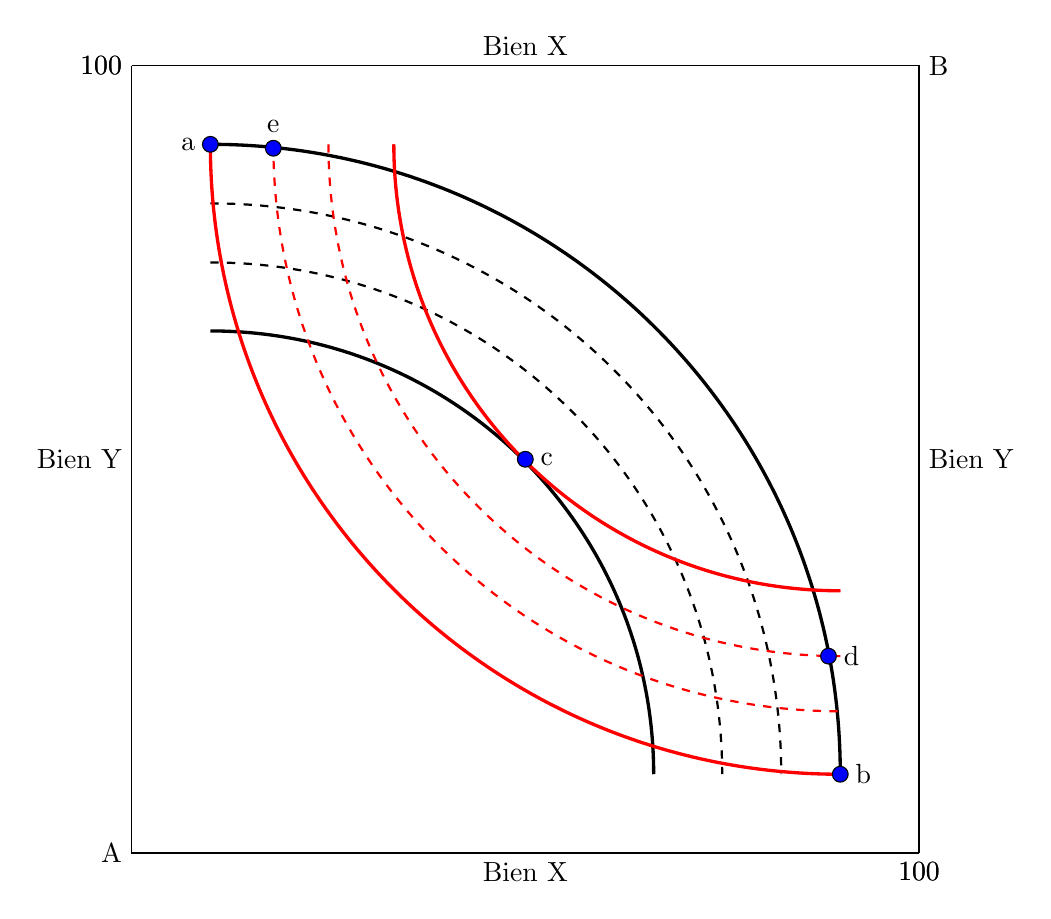
\begin{tikzpicture}
        \draw (0,10) node[left] {100} -- (0,0) node[midway,left] {Bien Y} node[left]{A} -- (10,0) node[midway,below] {Bien X} node[below] {100};
        \draw (0,10) node[left] {100} -- (10,10) node[midway,above] {Bien X} node[right]{B} -- (10,0) node[midway,right] {Bien Y} node[below] {100};

        \draw[very thick] (1, 9) to[out=0,in=90] (9, 1);
        \draw[very thick] (1, 6.63) to[out=0,in=90] (6.63, 1);
        \draw[thick,dashed] (1, 7.5) to[out=0,in=90] (7.5, 1);
        \draw[thick,dashed] (1, 8.25) to[out=0,in=90] (8.25, 1);
        \draw[thick,dashed,red] (3.33, 9) to[out=-90,in=180] (9, 3.33);

        \draw[very thick,red] (1, 9) to[out=-90,in=180] (9, 1);
        \draw[thick,dashed,red] (1.8, 9) to[out=-90,in=180] (9, 1.8);
        \draw[thick,dashed,red] (2.5, 9) to[out=-90,in=180] (9, 2.5);
        \draw[very thick,red] (3.33, 9) to[out=-90,in=180] (9, 3.33);

        \draw[fill=blue] (1,9) circle (1mm) node[left=2pt] {a};
        \draw[fill=blue] (9,1) circle (1mm) node[right=2pt] {b};
        \draw[fill=blue] (5,5) circle (1mm) node[right=2pt] {c};
        \draw[fill=blue] (8.85,2.5) circle (1mm) node[right=2pt] {d};
        \draw[fill=blue] (1.8,8.95) circle (1mm) node[above=2pt] {e};

    \end{tikzpicture}
    \end{center}

    \textbf{1.} Dans la boîte de Edgeworth ci-dessus, quelles sont les allocations
        Pareto-efficaces ?
        \begin{enumerate}
            \item Il n'y a pas d'allocation Pareto-efficace représentée
            \item \textsc{a} et \textsc{b}
            \item \textsc{c}
            \item \textsc{d}
	    \end{enumerate}


    \textbf{2.} Dans la boîte de Edgeworth ci-dessus, quelles sont les allocations
        Pareto-améliorantes par rapport à \textsc{e} ?
        \begin{enumerate}
            \item \textsc{a}, \textsc{d} et \textsc{b}
            \item \textsc{c}
            \item \textsc{d}
            \item \textsc{c} et \textsc{d}
	    \end{enumerate}

    \section{Correction}

    \subsection{} Pour qu'une allocation soit améliorante au sens de Pareto, il faut (par
    définition de ce qu'est une amélioration au sens de Pareto) que l'utilité
    des deux agents soit au moins aussi élevée que dans l'allocation initiale
    (personne n'est lésés) et que l'utilité d'au moins un des deux agents soit
    plus élevée.

    Dans l'allocation initiale, \(u_a = 5 * 3 = 15\) et \(u_b = 5*7 = 35\)

    Autrement, on cherche une allocation telle que :
    \begin{itemize}
        \item \(u_a = 15\) et \(u_b > 35\),
        \item ou \(u_a > 15\) et \(u_b = 35\)
        \item ou \(u_a > 15\) et \(u_b > 35\)
    \end{itemize}

    L'allocation \(4\) est Pareto améliorante, puisque \(u_a = 16 > 15\) et
    \(u_b = 36 > 35\).

    \subsection{}
        \[TMS_{x,y} = \frac{\frac{\partial U}{\partial x}}{\frac{\partial U
        }{\partial y}} = \frac{2x}{2y} = \frac{x}{y} \]


   \textbf{4.} Laquelle des propositions suivantes énonce le second théorème du bien-être ?
	    \begin{enumerate}
	    \item Toute allocation Pareto optimale est efficace.
	    \item Toute allocation d'équilibre concurrentiel est un optimum de Pareto.
	    \item Toute allocation d'équilibre concurrentiel peut être rendue équitable
              après avoir réalisé les transferts adéquats.
	    \item Toute allocation Pareto optimale peut être obtenue comme équilibre
        concurrentiel après réallocation adéquate des dotations initiales.
	    \end{enumerate}



    \textbf{2.} Dans la boîte de Edgeworth, que représente la courbe des contrats ?
	    \begin{enumerate}
	    \item Les allocations Pareto-améliorantes
	    \item Les allocations Pareto-efficaces
	    \item Les courbes d'indifférence des deux agents
	    \item Les allocations qui maximisent le bien-être social
	    \end{enumerate}

	\textbf{3.} Comment est défini le surplus du consommateur ?
		\begin{enumerate}
		\item C'est l'utilité marginale procurée par la consommation d'un bien
        \item C'est la somme des écarts entre le prix de réserve du bien et le
              prix payé pour se le procurer, pour chaque unité du bien consommée
		\end{enumerate}

	\textbf{4.} Le critère de Pareto permet-il de classer entre elles toutes
                les situations possibles ?
		\begin{enumerate}
		\item Oui
        \item Non
		\end{enumerate}


    \textbf{1.} Quelles sont les principales critiques de l'utilitarisme ?

    \textbf{2.} Le maximin rawlsien est-il compatible avec une distribution
                inégalitaire des revenus ?

    \textbf{1.} Quelles sont les principales critiques de l'utilitarisme ?

    \dotfill

    \begin{itemize}
        \item Impossibilité pratique de mesurer l'utilité
        \item Poids identique accordé à tous les individus indépendemment de
            leurs caractéristiques (par exemple, pas de considération
            particulière pour les plus pauvres en tant que tels)
        \item Pas de jugement sur la manière dont l'utilité est procurée, i.e.\
            deux activités qui procurent la même utilité sont jugées aussi
            bonnes (e.g.\ persécuter une minorité peut donc être optimal)
        \item Pas de considération pour les droits fondamentaux en dehors de
            l'utilité qu'ils pourraient apporter
    \end{itemize}

    \dotfill

    \textbf{2.} Le maximin rawlsien est-il compatible avec une distribution
                inégalitaire des revenus ?

    \dotfill

    Oui, tant que cette distribution améliore le sort du moins bien loti.
    Une allocation qui améliore le sort du moins bien loti mais augmente les
    inégalités est donc positive au sens du maximin.

    \dotfill



    On étudie une économie avec deux agents, \(A\) et \(B\), et deux biens, \(\gamma\)
    et \(\delta\).

    La quantité totale du bien \(\gamma\) est de 5 unités et celle du bien \(\delta\)
    est de 10 unités.

    On note \(\gamma_{A}\) la quantité du bien \(\gamma\) détenue par l'individu
    \(A\), \(\delta_{A}\) la quantité du bien \(\delta\) détenue par l'individu
    \(A\), \(\gamma_{B}\) la quantité du bien \(\gamma\) détenue par l'individu
    \(B\), et \(\delta_{B}\) la quantité du bien \(\delta\) détenue par l'individu
    \(B\).

    Les deux agents ont pour fonction d'utilité respectivement \(U_{A}\left(\gamma_{A},
    \delta_{A}\right) = \gamma_{A} + \delta_{A}^{1/2}\) et
    \(U_{B}\left(\gamma_{B}, \delta_{B}\right) = \gamma_{B}^{1/2} + \delta_{B}\)


    L'allocation initale des biens est de 3 unités du bien \(\gamma\) et 4 unités du bien \(\delta\) pour \(A\),
    que l'on note \(A = \left(3,4\right)\), et de \(B = \left(2,6\right)\).

    \textbf{1.} Représentez cette économie par une boîte de Edgeworth

    \textbf{2.} Représentez les courbes d'indifférence sur lesquels se placent les deux individus

    \textbf{3.} L'allocation initiale est-elle Pareto-efficace ? Si non, quelles sont les allocations Pareto-améliorantes ?

    \textbf{4.} Déterminez une allocation Pareto-efficace. Calculez le taux marginal de substitution des deux agents en ce point. Quelle propriété satisfont-ils ?

    \textbf{5.} L'allocation initiale respecte-t'elle le principe rawlsien du maximin ?

    \textbf{A2.}

    On étudie une économie de 10 agents, numérotés de 1 à 10, dont les revenus
    du travail sont :

    \begin{table}[h!]
        \centering
        \begin{tabular}{c|cccccccccc}
            Individu & 1 & 2 & 3 & 4  & 5  & 6  & 7  & 8  & 9  & 10 \\ \hline
            Revenu   & 0 & 0 & 5 & 10 & 10 & 20 & 30 & 40 & 50 & 85
        \end{tabular}
    \end{table}

    \textbf{1.} Quel est le revenu moyen ? Quel est le revenu médian ?

    \textbf{2.} Tracez la courbe de Lorenz pour le revenu dans cette économie.

    Supposez que tous les agents ont une fonction d'utilité
    \(U\left(R\right) = R^{1/2}\).

    \textbf{3.} Quels transferts faudrait-il mettre en place pour maximiser une
    fonction de bien-être social utilitariste ?

    \textbf{4.} Quelle répartition des revenus vous semble la plus juste dans
    cette économie ?


    \textbf{A1.}

    On étudie une économie avec deux agents, \(A\) et \(B\), et deux biens, \(\gamma\)
    et \(\delta\).

    La quantité totale du bien \(\gamma\) est de 5 unités et celle du bien \(\delta\)
    est de 10 unités.

    On note \(\gamma_{A}\) la quantité du bien \(\gamma\) détenue par l'individu
    \(A\), \(\delta_{A}\) la quantité du bien \(\delta\) détenue par l'individu
    \(A\), \(\gamma_{B}\) la quantité du bien \(\gamma\) détenue par l'individu
    \(B\), et \(\delta_{B}\) la quantité du bien \(\delta\) détenue par l'individu
    \(B\).

    Les deux agents ont pour fonction d'utilité respectivement \(U_{A}\left(\gamma_{A},
    \delta_{A}\right) = \gamma_{A} + \delta_{A}^{1/2}\) et
    \(U_{B}\left(\gamma_{B}, \delta_{B}\right) = \gamma_{B}^{1/2} + \delta_{B}\)

    L'allocation initale des biens est de 3 unités du bien \(\gamma\) et 4 unités du bien \(\delta\) pour \(A\),
    que l'on note \(A = \left(3,4\right)\), et de \(B = \left(2,6\right)\).

    \textbf{1.} Représentez cette économie par une boîte de Edgeworth

    \textbf{2.} Représentez les courbes d'indifférence sur lesquels se placent les deux individus

    \dotfill

    Cf.\ graphes.

    \begin{figure}[p]
        \centering
        \includegraphics[width=8cm]{allocation_initiale}
        \includegraphics[width=8cm]{indifference_a}
        \includegraphics[width=8cm]{indifference_b}
        \caption{Représentation graphique de l'économie}
    \end{figure}

    \dotfill

    \textbf{3.} L'allocation initiale est-elle Pareto-efficace ? Si non, quelles sont les allocations Pareto-améliorantes ?

    \dotfill

    Non : toutes les allocations dans la lentille en haut à gauche de
    l'allocation initiale sont des améliorations au sens de Pareto :
    \begin{itemize}
        \item le long de la courbe d'indifférence de \(A\) (en orange),
            l'utilité de \(A\) est inchangée et celle de \(B\) est plus élevée
        \item le long de la courbe d'indifférence de \(B\) (en bleu),
            l'utilité de \(B\) est inchangée et celle de \(A\) est plus élevée
        \item entre les deux courbes, l'utilité des deux agents augmente
    \end{itemize}

    \dotfill

    \textbf{4.} Déterminez une allocation Pareto-efficace. Calculez le taux
    marginal de substitution des deux agents en ce point. Quelle propriété satisfont-ils ?

    \dotfill

    Trivialement, les allocations où tous les biens sont possédés par \(A\) ou
    par \(B\) sont Pareto-efficaces.

    On peut également partir de la définition de l'équilibre (la demande totale
    pour chacun des deux biens est égale à l'offre) ou d'une de ses propriétés
    (les taux marginaux de substitution sont égaux à l'équilibre) pour trouver
    un équilibre : or, comme toutes les équilibres concurrentiels sont efficaces
    au sens de Pareto, cela correspond à une allocation Pareto-efficace.

    Partons de l'allocation \(A = \left(4, 1\right)\) et \(B = \left(1, 9\right)\) (pour se simplifier les calculs
    et notamment éviter les cas particuliers où la consommation optimale d'un bien est
    négative). Le raisonnement est le même quelque soit l'allocation de départ.

    Notons \(p_{\delta}\) le prix d'équilibre du bien \(\delta\) exprimé en unités
    du bien \(\gamma\). Notons \(p_{\gamma}\) le prix d'équilibre du bien \(\gamma\)
    exprimé en unités du bien \(\gamma\). On a donc \(p_{\gamma} = 1\). On appelle
    alors le bien \(\gamma\) le numéraire.

    Plus généralement, si \(\left(p'_{\delta}, p'_{\gamma}\right)\) sont les prix
    d'équilibre, alors pour tout \(\Phi > 0\), \(\left(p'_{\delta} / \Phi, p'_{\gamma} / \Phi \right)\)
    sont également des prix d'équilibre. Par souci de clarté, on fixe un des prix
    à 1 (le prix du bien numéraire). Ici, on prend \(\Phi = p'_{\gamma}\) et le vecteur
    des prix d'équilibre est donc \(\left(p'_{\delta} / p'_{\gamma}, p'_{\gamma} / p'_{\gamma} \right) = \left(p_{\delta}, 1\right)\).

    Compte tenu de ces prix d'équilibre et de l'allocation initiale, la valeur
    des biens détenus par \(A\) est :
    \[ R_{A} = \gamma^{\text{initial}}_{A} \times p_{\gamma} + \delta^{\text{initial}}_{A} \times p_{\delta} = 4 \times 1 + 1 \times p_{\delta} = 4 + p_{\delta} \]

    La valeur de son panier de consommation est :
    \[ \gamma_{A} \times p_{\gamma} + \delta_{A} \times p_{\delta} = \gamma_{A}  + \delta_{A} \times p_{\delta} \]

    À l'optimum, la contrainte de budget sera saturée : 
    \[ \gamma_{A}  + \delta_{A} \times p_{\delta}  = 4 + p_{\delta} \Rightarrow \gamma_{A} = 4 + p_{\delta} - \delta_{A} p_{\delta} \]

    L'individu \(A\) maximise son utilité :
    \[ \max U_{A} = \gamma_{A} + \delta_{A}^{1/2} =  4 + p_{\delta} - \delta_{A} p_{\delta} + \delta_{A}^{1/2}\]

    Au maximum, la dérivée de \(U_{A}\) par rapport à la variable de choix (\(\delta_{A}\)) est nulle :
    \begin{multline*}
         \frac{dU_{A}}{d\delta_{A}} = - p_{\delta} + \frac{1}{2\sqrt{\delta_{A}}} = 0 \\
        \Rightarrow \delta_{A} = \frac{1}{4p_{\delta}^{2}} \\
        \Rightarrow \gamma_{A} = 4 + p_{\delta} - \frac{1}{4p_{\delta}}
    \end{multline*}

    On procède de la même manière pour l'individu \(B\) (i.e.\ on exprime son
    revenu, sa contrainte de budget et on maximise son utilité sous containte), et
    l'on obtient :
    \begin{align*}
        \gamma_{B} &= \frac{1}{4} p_{\delta}^{2}\\
        \delta_{B} &= \frac{1}{p_{\delta}} - \frac{1}{4} p_{\delta} + 9\\
    \end{align*}

    Nous avons donc les offres totales en \(\gamma\) et en \(\delta\) (qui sont
    fixes et données dans l'énoncé), ainsi que les demandes totales en \(\gamma\)
    et en \(\delta\), qui sont respectivement \(\gamma_{A} + \gamma_{B}\) et
    \(\delta_{A} + \delta_{B}\).

    À l'équilibre (par définition de ce qu'est l'équilibre), l'offre est égale
    à la demande pour chacun des biens :
    \begin{align*}
        5 &= \gamma_{A} + \gamma_{B} &=  4 + p_{\delta} - \frac{1}{4p_{\delta}} + \frac{1}{4p_{\delta}^{2}} \\
        10 &= \delta_{A} + \delta_{B} &=  \frac{1}{4p_{\delta}^{2}} +  \frac{1}{p_{\delta}} - \frac{1}{4} p_{\delta} + 9
    \end{align*}

    À partir de ces équations, il est possible de calculer le prix \(p_{\delta}\) d'équilibre.

    Partons de la seconde équation :
    \begin{align*}
        & 10 = \frac{1}{4p_{\delta}^{2}} +  \frac{1}{p_{\delta}} - \frac{1}{4} p_{\delta} + 9 \\
        \Rightarrow & 1 =  \frac{1}{4p_{\delta}^{2}} +  \frac{1}{p_{\delta}} - \frac{1}{4} p_{\delta} \\
        \Rightarrow & \frac{1}{4p_{\delta}^{2}} +  \frac{1}{p_{\delta}} - \frac{1}{4} p_{\delta} - 1 = 0 \\
        \Rightarrow & \frac{1}{4} +  p_{\delta} - \frac{1}{4} p_{\delta}^{3} - p_{\delta}^{2} = 0 \\
        \Rightarrow & 1 +  4 p_{\delta} -  p_{\delta}^{3} - 4 \times p_{\delta}^{2} = 0 \\
    \end{align*}

    À partir de la dernière ligne, on peut résoudre à la main l'équation ou \href{https://www.wolframalpha.com/input/?i=solve+1+%2B+4x+-+x%5E3+-+4x%5E2+%3D+0}{via
    son ordinateur} et on trouve \(p_{\delta} = 1\).

    On peut en déduire toutes les quantités d'équilibre :
    \begin{align*}
        \gamma_{A} &= 4 + p_{\delta} - \frac{1}{4p_{\delta}} &= 4 + 1 - \frac{1}{4} &= 5 - \frac{1}{4} \\
        \delta_{A} &= \frac{1}{4p_{\delta}^{2}}  &= \frac{1}{4}\\
        \gamma_{B} &= \frac{1}{4} p_{\delta}^{2} &= \frac{1}{4}\\
        \delta_{B} &= \frac{1}{p_{\delta}} - \frac{1}{4} p_{\delta} + 9 &= 1 - \frac{1}{4} + 9 &= 10 - \frac{1}{4}
    \end{align*}

    D'après le premier théorème du bien-être l'allocation \(A = \left( 5 - \frac{1}{4}, \frac{1}{4} \right) \) et
    \( B = \left( \frac{1}{4}, 10 - \frac{1}{4} \right) \) est Pareto-efficace.

    On peut en déduire les taux marginaux de substitution en ce point :
    \begin{align*}
        TMS_{\gamma,\delta}^{A} &= \frac{\partial U_{A}}{\partial \gamma_{A}} / \frac{\partial U_{A}}{\partial \delta_{A}} = \frac{1}{\frac{1}{2\sqrt{\frac{1}{4}}}} = 2 \sqrt{\frac{1}{4}} = 2 \times \frac{1}{2} &= 1 \\
        TMS_{\gamma,\delta}^{B} &= \frac{\partial U_{B}}{\partial \gamma_{B}} / \frac{\partial U_{B}}{\partial \delta_{B}} = \frac{\frac{1}{2\sqrt{\frac{1}{4}}}}{1} = \frac{1}{2\sqrt{\frac{1}{4}}} = \frac{1}{2 \times \frac{1}{2}} &= 1 \\
        \frac{p_{\gamma}}{p_{\delta}} &= \frac{1}{1} &= 1
    \end{align*}

    Au point d'équilibre qui est aussi une allocation Pareto-efficace, les taux
    marginaux de substitution des deux agents sont égaux et égaux au ratio des
    prix. Graphiquement, les deux courbes
    d'indifférence et la droite de budget sont tangentes.
    
    \dotfill

    \textbf{5.} L'allocation initiale respecte-t'elle le principe rawlsien du maximin ?

    \dotfill

    L'utilité de l'individu qui a la plus basse utilité (\(A\)) est de 5.

    Pour l'allocation (par exemple) \(A = \left(5,1\right)\) et \(B =
    \left(0,9\right)\), l'utilité de l'individu qui a la plus basse utilité
    (toujours \(A\)) est maintenant de 6.

    L'allocation initiale ne maximise donc pas l'utilité de l'individu le moins
    bien loti.

    \dotfill

    \textbf{A2.}

    On étudie une économie de 10 agents, numérotés de 1 à 10, dont les revenus
    du travail sont :

    \begin{table}[h!]
        \centering
        \begin{tabular}{c|cccccccccc}
            Individu & 1 & 2 & 3 & 4  & 5  & 6  & 7  & 8  & 9  & 10 \\ \hline
            Revenu   & 0 & 0 & 5 & 10 & 10 & 20 & 30 & 40 & 50 & 85
        \end{tabular}
    \end{table}

    \textbf{1.} Quel est le revenu moyen ? Quel est le revenu médian ?

    \dotfill

    Le revenu moyen est de 25 et le revenu médian (revenu tel que la moitié des
    individus ont plus que ce revenu et l'autre moitié a moins) est de 15.

    \dotfill

    \textbf{2.} Tracez la courbe de Lorenz pour le revenu dans cette économie.

    \dotfill

    Cf.\ graphe.

    \begin{figure}[p]
        \centering
        \includegraphics[width=8cm]{lorenz}
        \caption{Courbe de Lorenz de cette économie}
    \end{figure}

    \dotfill

    Supposez que tous les agents ont une fonction d'utilité
    \(U\left(R\right) = R^{1/2}\).

    \textbf{3.} Quels transferts faudrait-il mettre en place pour maximiser une
    fonction de bien-être social utilitariste ?

    \dotfill

    Soient deux agents \(A\) et \(B\) tels que \(R_{A} > R_{B}\).

    Alors, l'utilité marginale de \(A\) est plus faible que celle de \(B\) :
    \[ \frac{dU_A}{R_{A}} = \frac{1}{2\sqrt{R_{A}}} < \frac{1}{2\sqrt{R_{B}}} = \frac{dU_B}{R_{B}} \]

    Ainsi, lorsque l'on transfert du revenu de \(A\) à \(B\) on modifie la somme \(U_A + U_B\) (et
    donc la fonction de bien-être social) de \( - \frac{dU_A}{R_{A}} + \frac{dU_B}{R_{B}} > 0\).

    Autrement dit, tout transfert des plus riches vers les plus pauvres augmente la somme
    des utilités.

    La fonciton de bien-être sociale est donc maximisée quand il n'est plus possible de l'augmenter,
    i.e.\ quand il n'y a plus de transfert des riches vers les pauvres possibles, i.e.\ lorsque
    tous les individus ont le même revenu.

    Il faut donc appliquer un transfert de \(25 - R_{i}\) à tous les individus, de telle sorte
    que le revenu de chacun soit, après transfert \(R_{i} + \left(25 - R_{i}\right) = 25\).


\end{document}
